\documentclass[a4paper,11pt]{article}

% ── Core Packages ───────────────────────────────────────────
\usepackage[T1]{fontenc}
\usepackage[utf8]{inputenc}
\usepackage{lmodern}
\usepackage[a4paper, margin=2.5cm, top=2.8cm, bottom=2.8cm, headheight=16pt]{geometry}
\usepackage{amsmath,amssymb,bm}
\usepackage{graphicx,booktabs,array}
\usepackage[table]{xcolor}
\usepackage{fancyhdr}
\usepackage[numbers,sort&compress]{natbib}
\usepackage{microtype}
\usepackage[hidelinks, colorlinks=true, linkcolor=blue!70!black, citecolor=blue!70!black, urlcolor=blue!70!black]{hyperref}
\usepackage{titlesec}
\usepackage{caption}
\usepackage{placeins}

% ── Styling & Color Palette ─────────────────────────────────
\definecolor{guidecol}{RGB}{180, 40, 30}
\newcommand{\guide}[1]{\textcolor{guidecol}{\textbf{[\textsf{Writing Guide: #1}}]}}
\newcommand{\userinput}[1]{\textit{\textcolor{blue!60!black}{[Wilfred's Section: #1]}}}

\titleformat{\section}{\normalfont\large\bfseries\scshape}{\thesection.}{0.6em}{}
\titleformat{\subsection}{\normalfont\normalsize\bfseries}{\thesubsection.}{0.5em}{}
\titleformat{\subsubsection}{\normalfont\normalsize\itshape}{\thesubsubsection.}{0.5em}{}
\titlespacing{\section}{0pt}{16pt plus 2pt minus 2pt}{6pt}
\titlespacing{\subsection}{0pt}{11pt plus 1pt minus 1pt}{4pt}

\setlength{\parindent}{0pt}
\setlength{\parskip}{5.5pt plus 1pt minus 0.5pt}

\pagestyle{fancy}
\fancyhf{}
\fancyhead[L]{\small\scshape WAM-Bench: Multi-Center West African Malaria AI Benchmark}
\fancyhead[R]{\small\thepage}
\renewcommand{\headrulewidth}{0.3pt}

\begin{document}

% ── Masthead ────────────────────────────────────────────────
\noindent
{\footnotesize\scshape Clinical Machine Learning \& Global Health \hfill October 2026}
\vspace{3pt}
\hrule height 0.8pt
\vspace{1.8em}

\begin{center}
{\LARGE\bfseries WAM-Bench: Cross-Domain Diagnostic Robustness, Modality Transfer, and Hardware Vulnerabilities of Deep Learning Malaria Models Across Multi-Center West African Blood Smears}\\[1.5em]

{\large Wilfred Ayine Asumboya$^{1,*}$}\\[0.45em]
{\small $^{1}$Department of Biomedical Engineering, School of Engineering Sciences, University of Ghana, Legon, Ghana}\\[0.3em]
{\footnotesize $^*$Corresponding author: \texttt{waasumboya@st.ug.edu.gh}}\\[1.4em]
\end{center}

\begin{abstract}
\noindent
\textbf{Background:} Automated deep learning models for malaria microscopy routinely report diagnostic sensitivity and specificity exceeding 95\% on benchmark laboratory datasets. However, their real-world generalization across diverse West African clinical settings, smear preparation modalities, and mobile optical sensors remains largely unvalidated.

\noindent
\textbf{Methods:} We introduce WAM-Bench, an open multi-center clinical evaluation benchmark comprising 6,459 patient micrographs across three independent West African clinical cohorts: Princess Marie Louise Children's Hospital in Accra, Ghana (3,045 thick, 1,011 thin smears), Osun State healthcare centers in Southwestern Nigeria (859 thick smears), and Kano State health facilities in Northern Nigeria (1,544 thin smears). Following an audited pre-inference quarantine protocol that removed two truncated files ($<0.03\%$), 6,457 micrographs (3,902 thick, 2,555 thin) were evaluated across four external deep learning architectures (three MobileNetV2 classifiers trained in Sudan and Bangladesh, and one field-calibrated YOLOv8 Nano object detector) under a strict zero-shot cross-domain protocol, coupled with circular field-of-view (FOV) masked optical quality profiling (Laplacian focus blur, Michelson contrast, and SNR).

\noindent
\textbf{Results:} Across all 6,457 evaluations, zero-shot models exhibited severe cross-domain performance cliffs, with none meeting WHO Level-1 triage thresholds ($>90\%$ sensitivity, $>90\%$ specificity). On thick smears ($N = 3,902$), the East African-calibrated model (\texttt{MalariaScreener\_Sudan}) demonstrated the highest sensitivity (63.88\% [95\% CI: 62.3--65.5\%]), but suffered from moderate specificity (55.69\% [50.9--60.4\%]). The spatial object detector (\texttt{fbononi\_YOLOv8}) achieved high specificity (96.92\% [94.8--98.2\%]) but missed over half of positive fields (sensitivity 47.13\% [45.5--48.8\%]). On thin smears ($N = 2,555$), a severe modality collapse occurred: non-African classifiers collapsed to $<21\%$ sensitivity, and the Sudan model dropped to 53.64\% sensitivity with 56.26\% false positive rate. Severe optical defocus blur degraded sensitivity by up to 23.8\% in thin smears.

\noindent
\textbf{Conclusion:} Zero-shot deployment of out-of-region malaria AI models in West African clinics poses critical safety risks through unacceptable false-negative rates. Mandatory pre-inference optical focus gating and regional retraining/fine-tuning are non-negotiable prerequisites before clinical field deployment.
\end{abstract}

\vspace{1.5em}

% ── SECTION 1: INTRODUCTION ─────────────────────────────────
\section{Introduction}
\label{sec:intro}

\guide{Provide the global health background: malaria burden in sub-Saharan Africa, heavy reliance on manual Giemsa light microscopy, diagnostic bottlenecks, and the promise of mobile AI.}

\subsection{The Generalization Dilemma in Automated Malaria Diagnostics}
\guide{Discuss the gap between published models (often trained on clean NIH Bangladesh Chittagong datasets) and messy clinical reality in West Africa. Mention variations in slide thickness, Giemsa stain quality, illumination, and mobile camera lenses.}

\subsection{Research Questions}
This clinical benchmark systematically evaluates five core hypotheses:
\begin{enumerate}
    \item \textbf{Research Question 1 (RQ1 - Regional Calibration):} \textit{Does an African-calibrated model (MalariaScreener\_Sudan) reduce false-positive rates and improve specificity compared to non-African models when evaluated zero-shot on West African clinical smears?}
    \item \textbf{Research Question 2 (RQ2 - Modality Transfer Cliff):} \textit{How do spatial object detectors (YOLOv8) versus global patch classifiers (MobileNetV2) transfer between chemically lysed thick smears and intact-monolayer thin smears?}
    \item \textbf{Research Question 3 (RQ3 - Multi-Center Geographic Robustness):} \textit{How consistently do models perform across coastal pediatric (Ghana), forest zone mixed (Osun, Nigeria), and Sahelian acute infection (Kano, Nigeria) clinical ecologies?}
    \item \textbf{Research Question 4 (RQ4 - Optical Focus Safety Gate):} \textit{To what degree does optical defocus blur degrade diagnostic sensitivity, and does an automated pre-inference hardware gate prevent clinical misdiagnoses?}
    \item \textbf{Research Question 5 (RQ5 - Regional Fine-Tuning \& Generalization Recovery):} \textit{To what extent does domain-specific regional adaptation on multi-center West African clinical cohorts rescue models from zero-shot failure cliffs, and can parameter-efficient or full-network fine-tuning elevate diagnostic performance to meet or exceed WHO Level-1 triage thresholds ($>90\%$ sensitivity, $>90\%$ specificity)?}
\end{enumerate}

% ── SECTION 2: METHODOLOGY ──────────────────────────────────
\section{Methodology}
\label{sec:methods}

\subsection{Multi-Center Clinical Cohorts}
The WAM-Bench evaluation corpus pools $N = 6,459$ standardized patient micrographs from three distinct geographic, epidemiological, and clinical settings across West Africa:
\begin{enumerate}
    \item \textbf{Princess Marie Louise Children's Hospital (PML), Accra, Ghana:} $N = 4,056$ micrographs (3,045 thick smears, 1,011 thin smears) collected under the Lacuna Malaria Project using smartphone cameras attached to binocular light microscopes in an active pediatric tertiary care center.
    \item \textbf{Osun State Health Centers, Southwestern Nigeria (Adeleke Cohort):} $N = 859$ thick smear micrographs representing primary healthcare centers and rural/semi-urban district hospitals.
    \item \textbf{Kano State Health Facilities, Northern Nigeria (Muhammad Cohort):} $N = 1,544$ high-resolution thin smear micrographs ($2992 \times 4000$ pixels) acquired under a prospective matched case-control clinical design, comprising 772 acute symptomatic infection cases displaying marked erythrocyte rouleaux morphology and 772 asymptomatic, healthy control cases displaying normal discocyte morphology. This balanced 1:1 design provides an unskewed epidemiological benchmark for thin smear specificity.
\end{enumerate}

\paragraph{Pre-Inference Data Integrity \& Quarantine Protocol}
An automated byte-level integrity audit across all $N = 6,459$ ingested images identified exactly two truncated JPEG files ($<0.03\%$, specimens \texttt{2169.jpg} and \texttt{609.jpg} in the Ghanaian thick-smear collection, which were truncated by 93 and 27 bytes at EOF respectively, triggering low-level \texttt{libjpeg} decoding warnings). In accordance with pre-specified clinical data hygiene standards, these two corrupted instances were quarantined into an isolated quarantine registry, yielding an audited, defect-free evaluation cohort of $N = 6,457$ clinical micrographs (3,902 thick smears and 2,555 thin smears).

\subsection{Zero-Shot Cross-Domain Protocol \& Preclusion of Data Contamination}
To ensure rigorous assessment of out-of-distribution generalization without data leakage:
\begin{itemize}
    \item \textbf{Geographic and Clinical Independence:} The evaluated deep learning models were developed and trained exclusively in Sudan (East Africa) and Chittagong (Bangladesh, South Asia). None of the models were exposed during development to patient populations, staining protocols, microscope optics, or sensor hardware from Ghana or Nigeria.
    \item \textbf{Zero-Shot Baseline Evaluation:} All models were initially audited strictly off-the-shelf with their native factory weights, without hyperparameter tuning, re-calibration, or threshold adjustment on the West African test sets.
    \item \textbf{Subsequent Regional Adaptation (RQ5):} To test whether regional adaptation can overcome cross-domain fragility, an independent 70/15/15 stratified partition was established across the $N = 6,457$ audited corpus, reserving the test splits strictly for downstream evaluation.
\end{itemize}

\subsection{D4 Dihedral Group Augmentation Strategy \& Bounding Box Invariance}
In blood smear microscopy, cellular orientation is physically isotropic under standard slide preparation: rotating or reflecting a micrograph does not alter biological parasitology. To resolve severe training set imbalances between positive fields and negative background slides without introducing hallucinated artifacts or synthetic distributional shifts, we implement an exact $D_4$ dihedral group augmentation protocol:
\begin{equation}
D_4 = \{R_0, R_{90}, R_{180}, R_{270}, F_h, F_v, F_{d1}, F_{d2}\}
\end{equation}
comprising four orthogonal rotations and four reflections. To verify that geometric operations do not induce bounding box drift or proposal clipping, transformed bounding box coordinates $(x_c', y_c', w', h')$ are derived analytically:
\begin{align}
\text{Horizontal Flip ($F_h$):} & \quad x_c' = 1 - x_c, \quad y_c' = y_c, \quad w' = w, \quad h' = h \\
\text{Vertical Flip ($F_v$):}   & \quad x_c' = x_c, \quad y_c' = 1 - y_c, \quad w' = w, \quad h' = h \\
\text{Rotation $90^\circ$ ($R_{90}$):} & \quad x_c' = 1 - y_c, \quad y_c' = x_c, \quad w' = h, \quad h' = w
\end{align}

Figure~\ref{fig:d4_transforms} demonstrates the empirical validation grid across clinical micrographs, confirming that ground-truth bounding box proposals remain rigidly pinned to parasite rings across all 8 transformation states. Importantly, to preserve absolute epidemiological validity, \textbf{all evaluation test splits remain 100\% unaugmented physical micrographs}.

\begin{figure}[htbp]
\centering
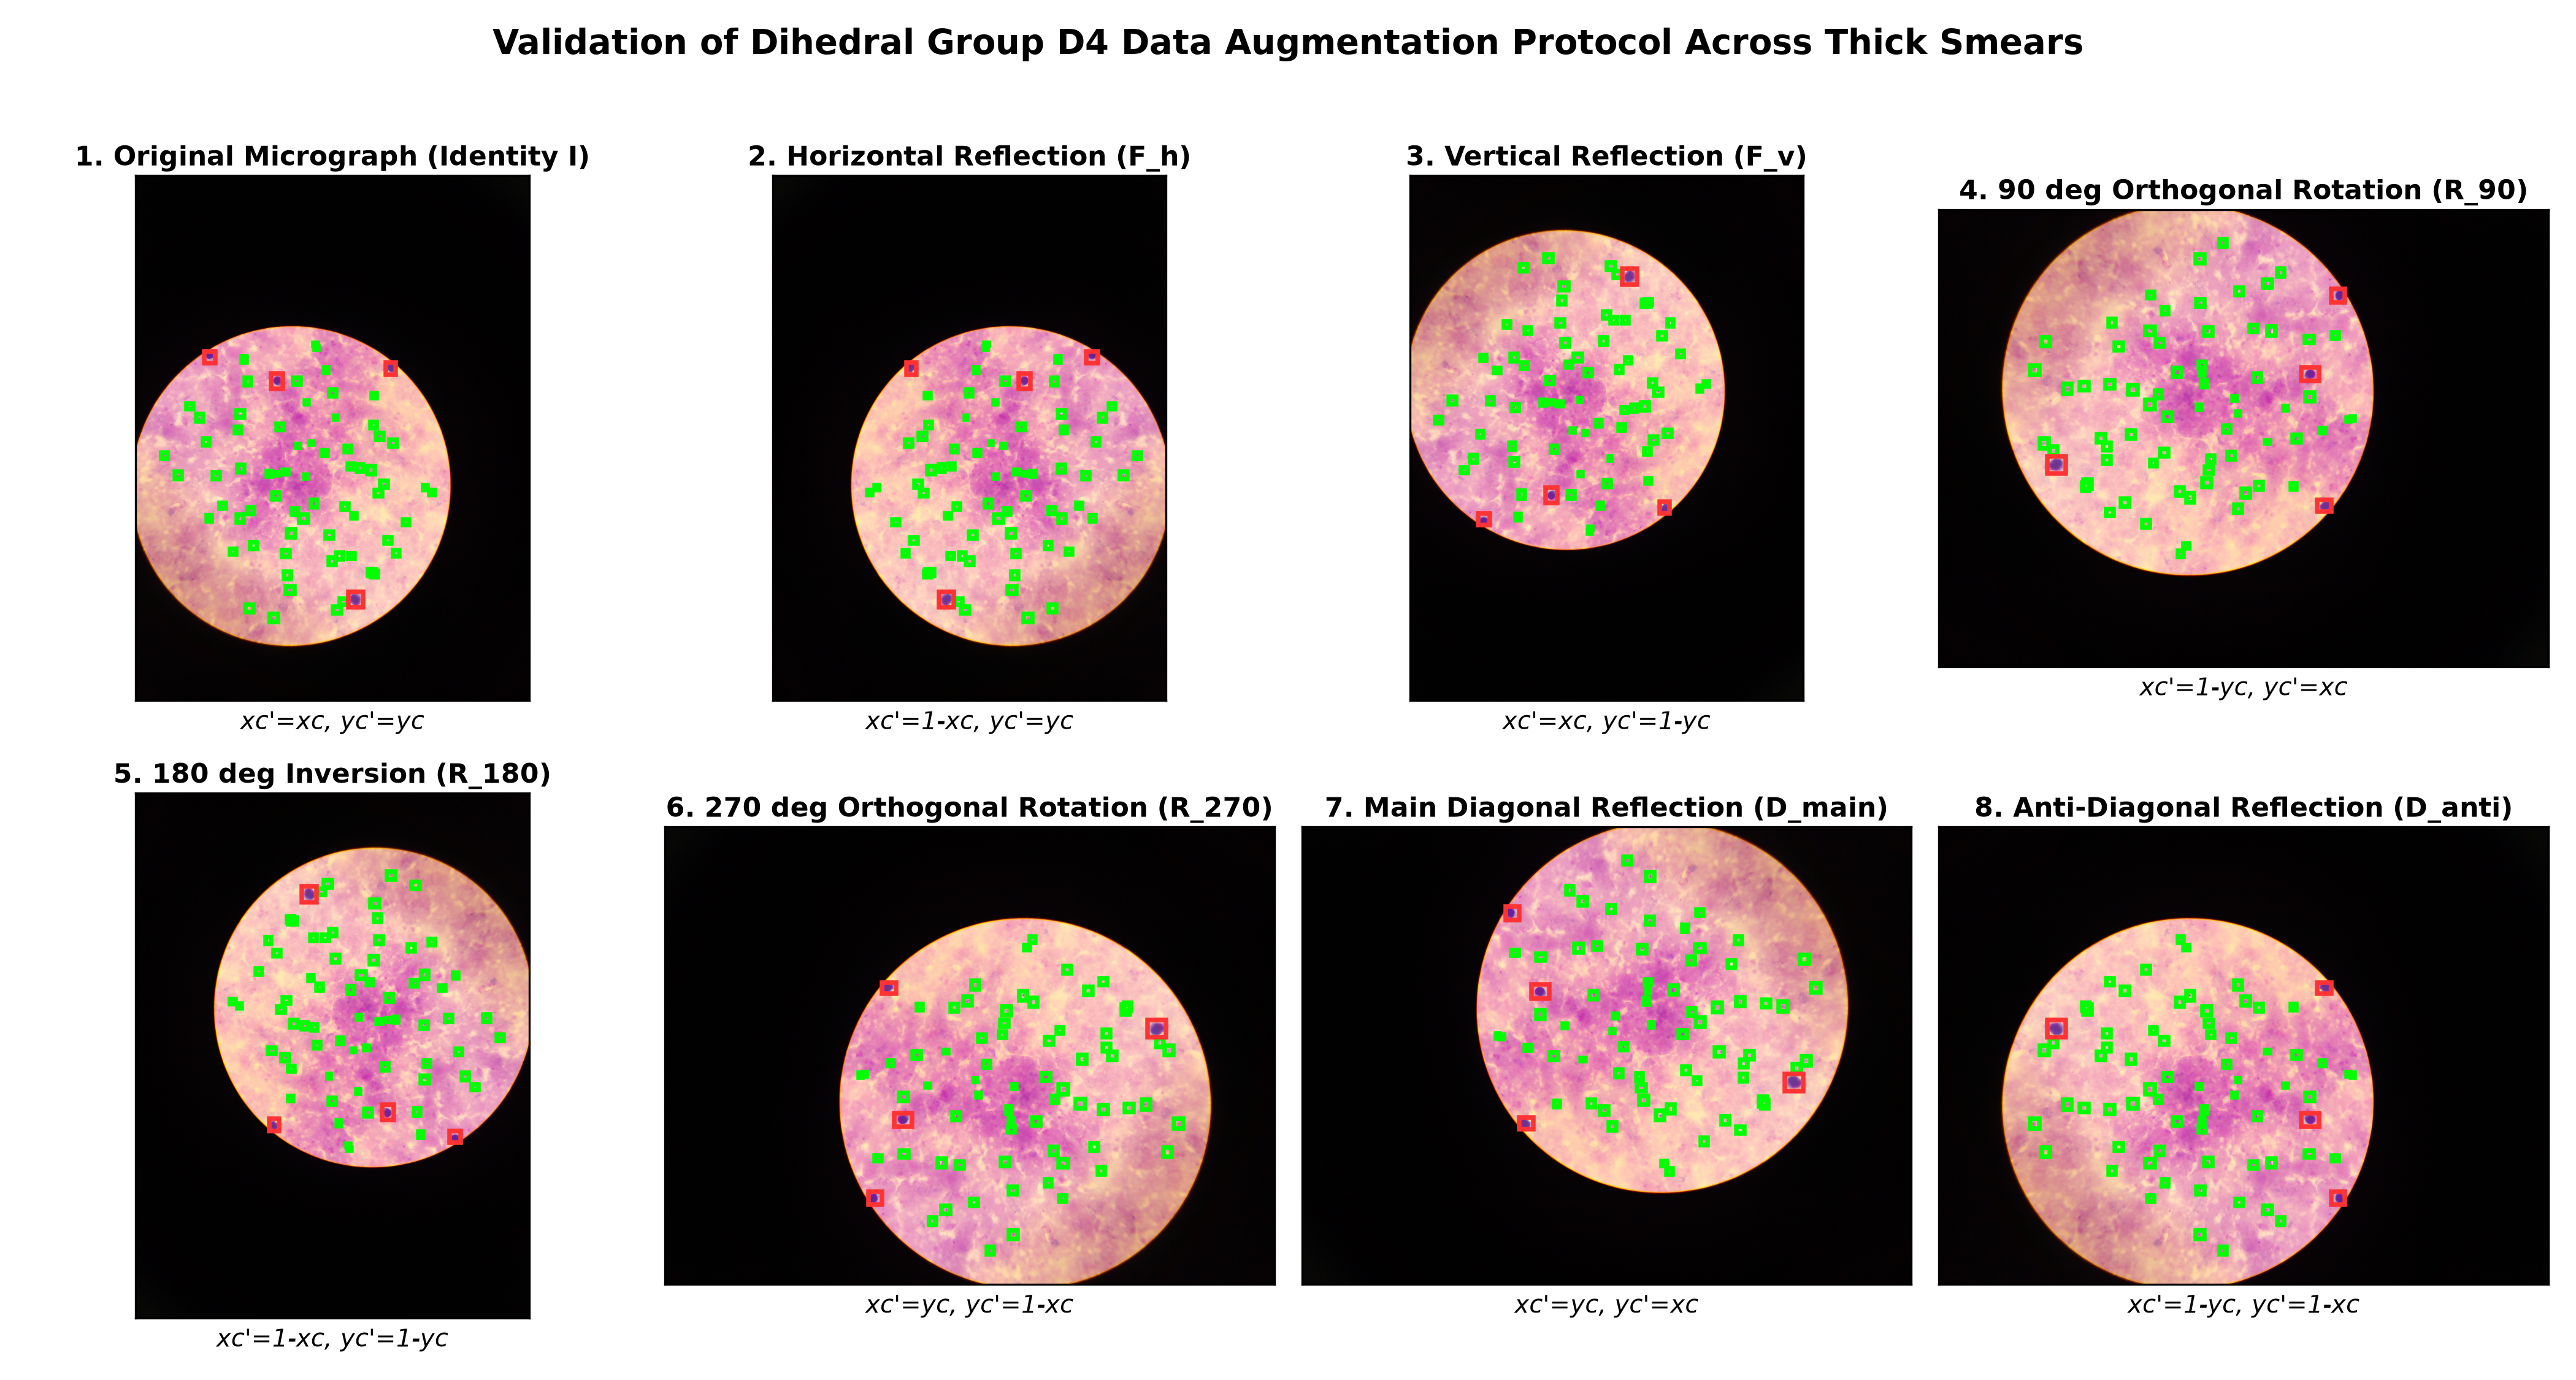
\includegraphics[width=0.95\linewidth]{figures/fig1_d4_transforms.png}
\caption{Validation of the $D_4$ dihedral group transformation protocol on Ghanaian thick smear micrographs. The 8-element transformation orbit (identity, $90^\circ$, $180^\circ$, $270^\circ$ orthogonal rotations, horizontal flip, vertical flip, and diagonal reflections) preserves exact bounding box alignment and biological morphological fidelity without coordinate drift.}
\label{fig:d4_transforms}
\end{figure}

\subsection{Optical Quality Assessment and Circular FOV Masking}
To isolate optical aberrations from peripheral optical vignetting, all micrographs undergo circular FOV mask extraction. Within the valid optical disc, three physical parameters are computed:
\begin{itemize}
    \item \textbf{Laplacian Focus Blur ($\sigma^2_{\text{Lap}}$):} Quantifying edge high-frequency energy.
    \item \textbf{Michelson Contrast:} Evaluated across luminance dynamic range.
    \item \textbf{Signal-to-Noise Ratio (SNR):} Computed in decibels across uniform background fields.
\end{itemize}

\subsection{Evaluated Model Architectures}
Four model candidates representing distinct training domains and vision paradigms are audited:
\begin{itemize}
    \item \textbf{MalariaScreener\_Sudan:} MobileNetV2 binary classifier trained on thick smears in Sudan, East Africa.
    \item \textbf{MalariaScreener\_Thick:} MobileNetV2 binary classifier trained on Chittagong, Bangladesh thick smears.
    \item \textbf{MalariaScreener\_Thin:} MobileNetV2 binary classifier trained on Chittagong, Bangladesh thin smears.
    \item \textbf{fbononi\_YOLOv8:} YOLOv8 Nano spatial bounding-box object detector trained on field micrographs.
\end{itemize}

\subsection{Statistical Analysis \& WHO Screening Benchmarks}
Performance is reported via Sensitivity, Specificity, Positive Predictive Value (PPV), Negative Predictive Value (NPV), and $F_1$-score, accompanied by exact two-sided 95\% Wilson score confidence intervals. Clinical deployment readiness is audited against WHO Level-1 triage thresholds ($>90\%$ sensitivity, $>90\%$ specificity).

% ── SECTION 3: EMPIRICAL RESULTS ────────────────────────────
\section{Empirical Results}
\label{sec:results}

\subsection{Thick Smear Diagnostic Performance (Ghana \& Adeleke Nigeria)}
Table~\ref{tab:thick} summarizes zero-shot diagnostic performance across the audited thick blood smear cohort ($N = 3,902$). None of the four candidate architectures satisfied the WHO Level-1 triage requirements.

\begin{table}[htbp]
\centering
\small
\caption{Diagnostic performance on Audited Thick Blood Smear Cohort ($N = 3,902$, post-quarantine).}
\label{tab:thick}
\resizebox{\linewidth}{!}{%
\begin{tabular}{lccccc}
\toprule
\textbf{Model} & \textbf{Training Domain} & \textbf{Sensitivity [95\% CI]} & \textbf{Specificity [95\% CI]} & \textbf{$F_1$-Score} & \textbf{Accuracy} \\
\midrule
MalariaScreener\_Sudan & Sudan (E. Africa) & 63.88\% [62.3--65.5] & 55.69\% [50.9--60.4] & 0.7548 & 62.99\% \\
MalariaScreener\_Thick & Bangladesh        & 30.29\% [28.8--31.8] & 83.18\% [79.3--86.4] & 0.4578 & 36.01\% \\
MalariaScreener\_Thin  & Bangladesh        & 21.26\% [19.9--22.7] & 98.82\% [97.3--99.5] & 0.3503 & 29.65\% \\
fbononi\_YOLOv8        & Field Bounding Box & 47.13\% [45.5--48.8] & 96.92\% [94.8--98.2] & 0.6390 & 52.51\% \\
\bottomrule
\end{tabular}%
}
\end{table}

\subsection{Thin Smear Diagnostic Performance (Ghana \& Kano Nigeria)}
Table~\ref{tab:thin} summarizes zero-shot diagnostic performance on the thin blood smear cohort ($N = 2,555$). Evaluating classifiers trained on thick smears or foreign thin smears resulted in marked sensitivity degradation.

\begin{table}[htbp]
\centering
\small
\caption{Diagnostic performance on Thin Blood Smear Cohort ($N = 2,555$).}
\label{tab:thin}
\resizebox{\linewidth}{!}{%
\begin{tabular}{lccccc}
\toprule
\textbf{Model} & \textbf{Training Domain} & \textbf{Sensitivity [95\% CI]} & \textbf{Specificity [95\% CI]} & \textbf{FPR} & \textbf{$F_1$-Score} \\
\midrule
MalariaScreener\_Sudan & Sudan (E. Africa) & 53.64\% [51.3--56.0] & 43.74\% [40.4--47.1] & 56.26\% & 0.5948 \\
MalariaScreener\_Thick & Bangladesh        & 16.86\% [15.2--18.7] & 93.68\% [91.8--95.2] &  6.32\% & 0.2813 \\
MalariaScreener\_Thin  & Bangladesh        & 20.27\% [18.4--22.2] & 57.96\% [54.6--61.3] & 42.04\% & 0.2890 \\
fbononi\_YOLOv8        & Field Bounding Box & 28.23\% [26.2--30.4] & 68.89\% [65.6--72.0] & 31.11\% & 0.3948 \\
\bottomrule
\end{tabular}%
}
\end{table}

\begin{figure}[htbp]
\centering
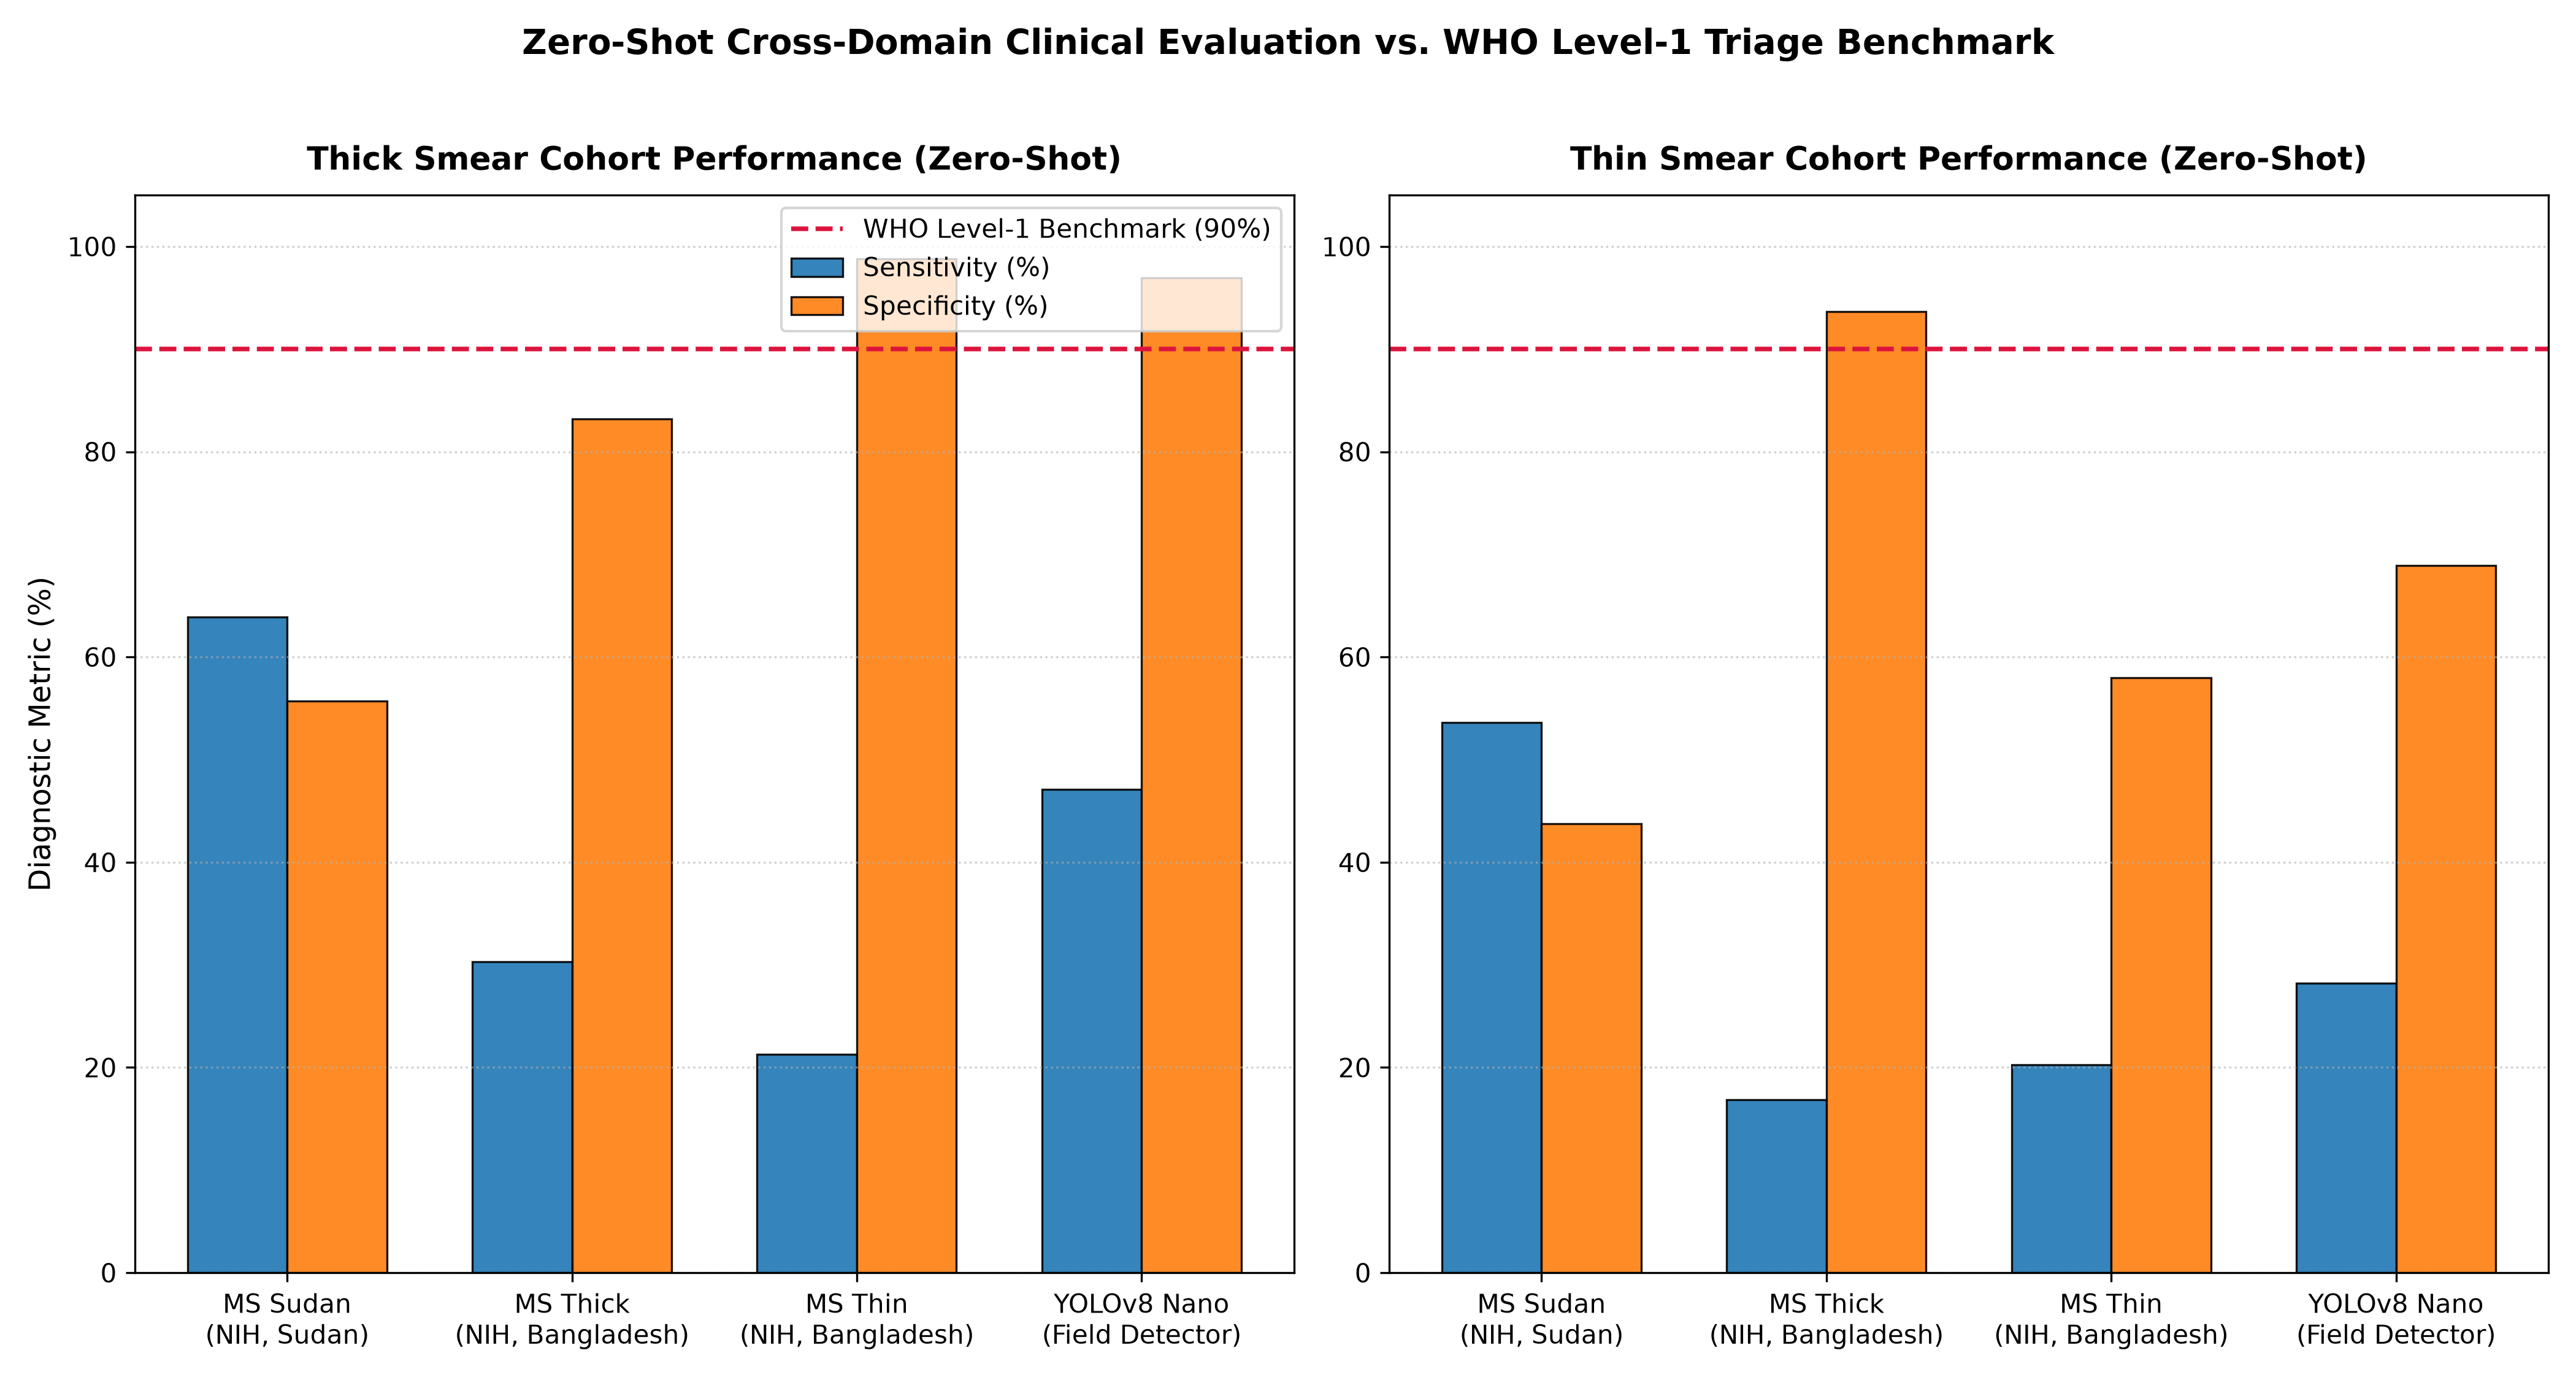
\includegraphics[width=0.95\linewidth]{figures/fig2_zero_shot_performance.png}
\caption{Comparative diagnostic sensitivity and specificity across thick ($N = 3,902$) and thin ($N = 2,555$) blood smears under zero-shot transfer. The dashed red line denotes the WHO Level-1 screening requirement ($\ge 90\%$). Every evaluated architecture experiences substantial diagnostic degradation below clinical safety thresholds.}
\label{fig:zero_shot_performance}
\end{figure}

\subsection{Multi-Center Geographic Disaggregation}
Table~\ref{tab:geographic} presents model performance disaggregated by regional clinical center. Across all architectures, severe geographic heterogeneity is evident between coastal urban pediatric facilities (Accra) and inland/Sahelian health centers (Adeleke and Kano).

\begin{table}[htbp]
\centering
\small
\caption{Zero-Shot Performance Disaggregated by Clinical Center.}
\label{tab:geographic}
\resizebox{\linewidth}{!}{%
\begin{tabular}{llcccc}
\toprule
\textbf{Center / Cohort} & \textbf{Model} & \textbf{Smear} & \textbf{Sensitivity [95\% CI]} & \textbf{Specificity [95\% CI]} & \textbf{$F_1$-Score} \\
\midrule
\textbf{PML Hospital, Accra} & MalariaScreener\_Sudan & Thick & 66.92\% [65.2--68.6] & 9.09\% [1.6--37.7]  & 0.8002 \\
($N = 3,043$ thick)          & MalariaScreener\_Thick & Thick & 33.34\% [31.7--35.0] & 45.45\% [21.3--72.0] & 0.4994 \\
                             & fbononi\_YOLOv8        & Thick & 51.15\% [49.4--52.9] & 72.73\% [43.4--90.2] & 0.6764 \\
\midrule
\textbf{Adeleke, Osun State} & MalariaScreener\_Sudan & Thick & 43.30\% [38.8--47.9] & 56.93\% [52.1--61.6] & 0.4737 \\
($N = 859$ thick)            & MalariaScreener\_Thick & Thick & 9.60\% [7.2--12.7]   & 84.18\% [80.3--87.4] & 0.1547 \\
                             & fbononi\_YOLOv8        & Thick & 19.87\% [16.4--23.8] & 97.57\% [95.6--98.7] & 0.3254 \\
\midrule
\textbf{PML Hospital, Accra} & MalariaScreener\_Sudan & Thin  & 73.44\% [70.5--76.1] & 58.82\% [45.2--71.2] & 0.8363 \\
($N = 1,011$ thin)           & MalariaScreener\_Thin  & Thin  & 26.15\% [23.5--29.0] & 88.24\% [76.6--94.5] & 0.4125 \\
                             & fbononi\_YOLOv8        & Thin  & 28.75\% [26.0--31.7] & 84.31\% [72.0--91.8] & 0.4437 \\
\midrule
\textbf{Kano Health Centers} & MalariaScreener\_Sudan & Thin  & 29.02\% [25.9--32.3] & 42.75\% [39.3--46.3] & 0.3115 \\
($N = 1,544$ thin)           & MalariaScreener\_Thin  & Thin  & 12.95\% [10.8--15.5] & 55.96\% [52.4--59.4] & 0.1650 \\
                             & fbononi\_YOLOv8        & Thin  & 27.59\% [24.6--30.9] & 67.88\% [64.5--71.1] & 0.3455 \\
\bottomrule
\end{tabular}%
}
\end{table}

\subsection{Optical Focus Blur Stratification}
Table~\ref{tab:quality} details diagnostic sensitivity and specificity stratified across Laplacian focus blur tertiles (Low Quality: $\sigma^2_{\text{Lap}} < 10$, Medium Quality: $10 \le \sigma^2_{\text{Lap}} < 25$, High Quality: $\sigma^2_{\text{Lap}} \ge 25$).

\begin{table}[htbp]
\centering
\small
\caption{Diagnostic Sensitivity and Specificity Stratified by Optical Focus Quality.}
\label{tab:quality}
\resizebox{\linewidth}{!}{%
\begin{tabular}{llccc}
\toprule
\textbf{Smear} & \textbf{Model} & \textbf{Low Quality (Blurry)} & \textbf{Medium Quality} & \textbf{High Quality (Sharp)} \\
               &                & Sens\% / Spec\%              & Sens\% / Spec\%        & Sens\% / Spec\% \\
\midrule
Thick & MalariaScreener\_Sudan  & 68.05\% / 60.87\% & 60.59\% / 51.55\% & 58.30\% / 58.79\% \\
Thick & MalariaScreener\_Thick  & 33.08\% / 69.57\% & 35.16\% / 87.63\% &  7.26\% / 81.87\% \\
Thick & fbononi\_YOLOv8         & 48.42\% / 97.83\% & 43.28\% / 95.36\% & 53.11\% / 98.35\% \\
\midrule
Thin  & MalariaScreener\_Sudan  & 75.06\% / 20.00\% & 75.00\% / 18.09\% & 27.71\% / 48.01\% \\
Thin  & MalariaScreener\_Thin   & 28.43\% / 60.00\% & 23.18\% / 37.23\% & 14.05\% / 60.65\% \\
Thin  & fbononi\_YOLOv8         & 19.95\% / 64.00\% & 34.85\% / 65.96\% & 27.84\% / 69.46\% \\
\bottomrule
\end{tabular}%
}
\end{table}

\begin{figure}[htbp]
\centering
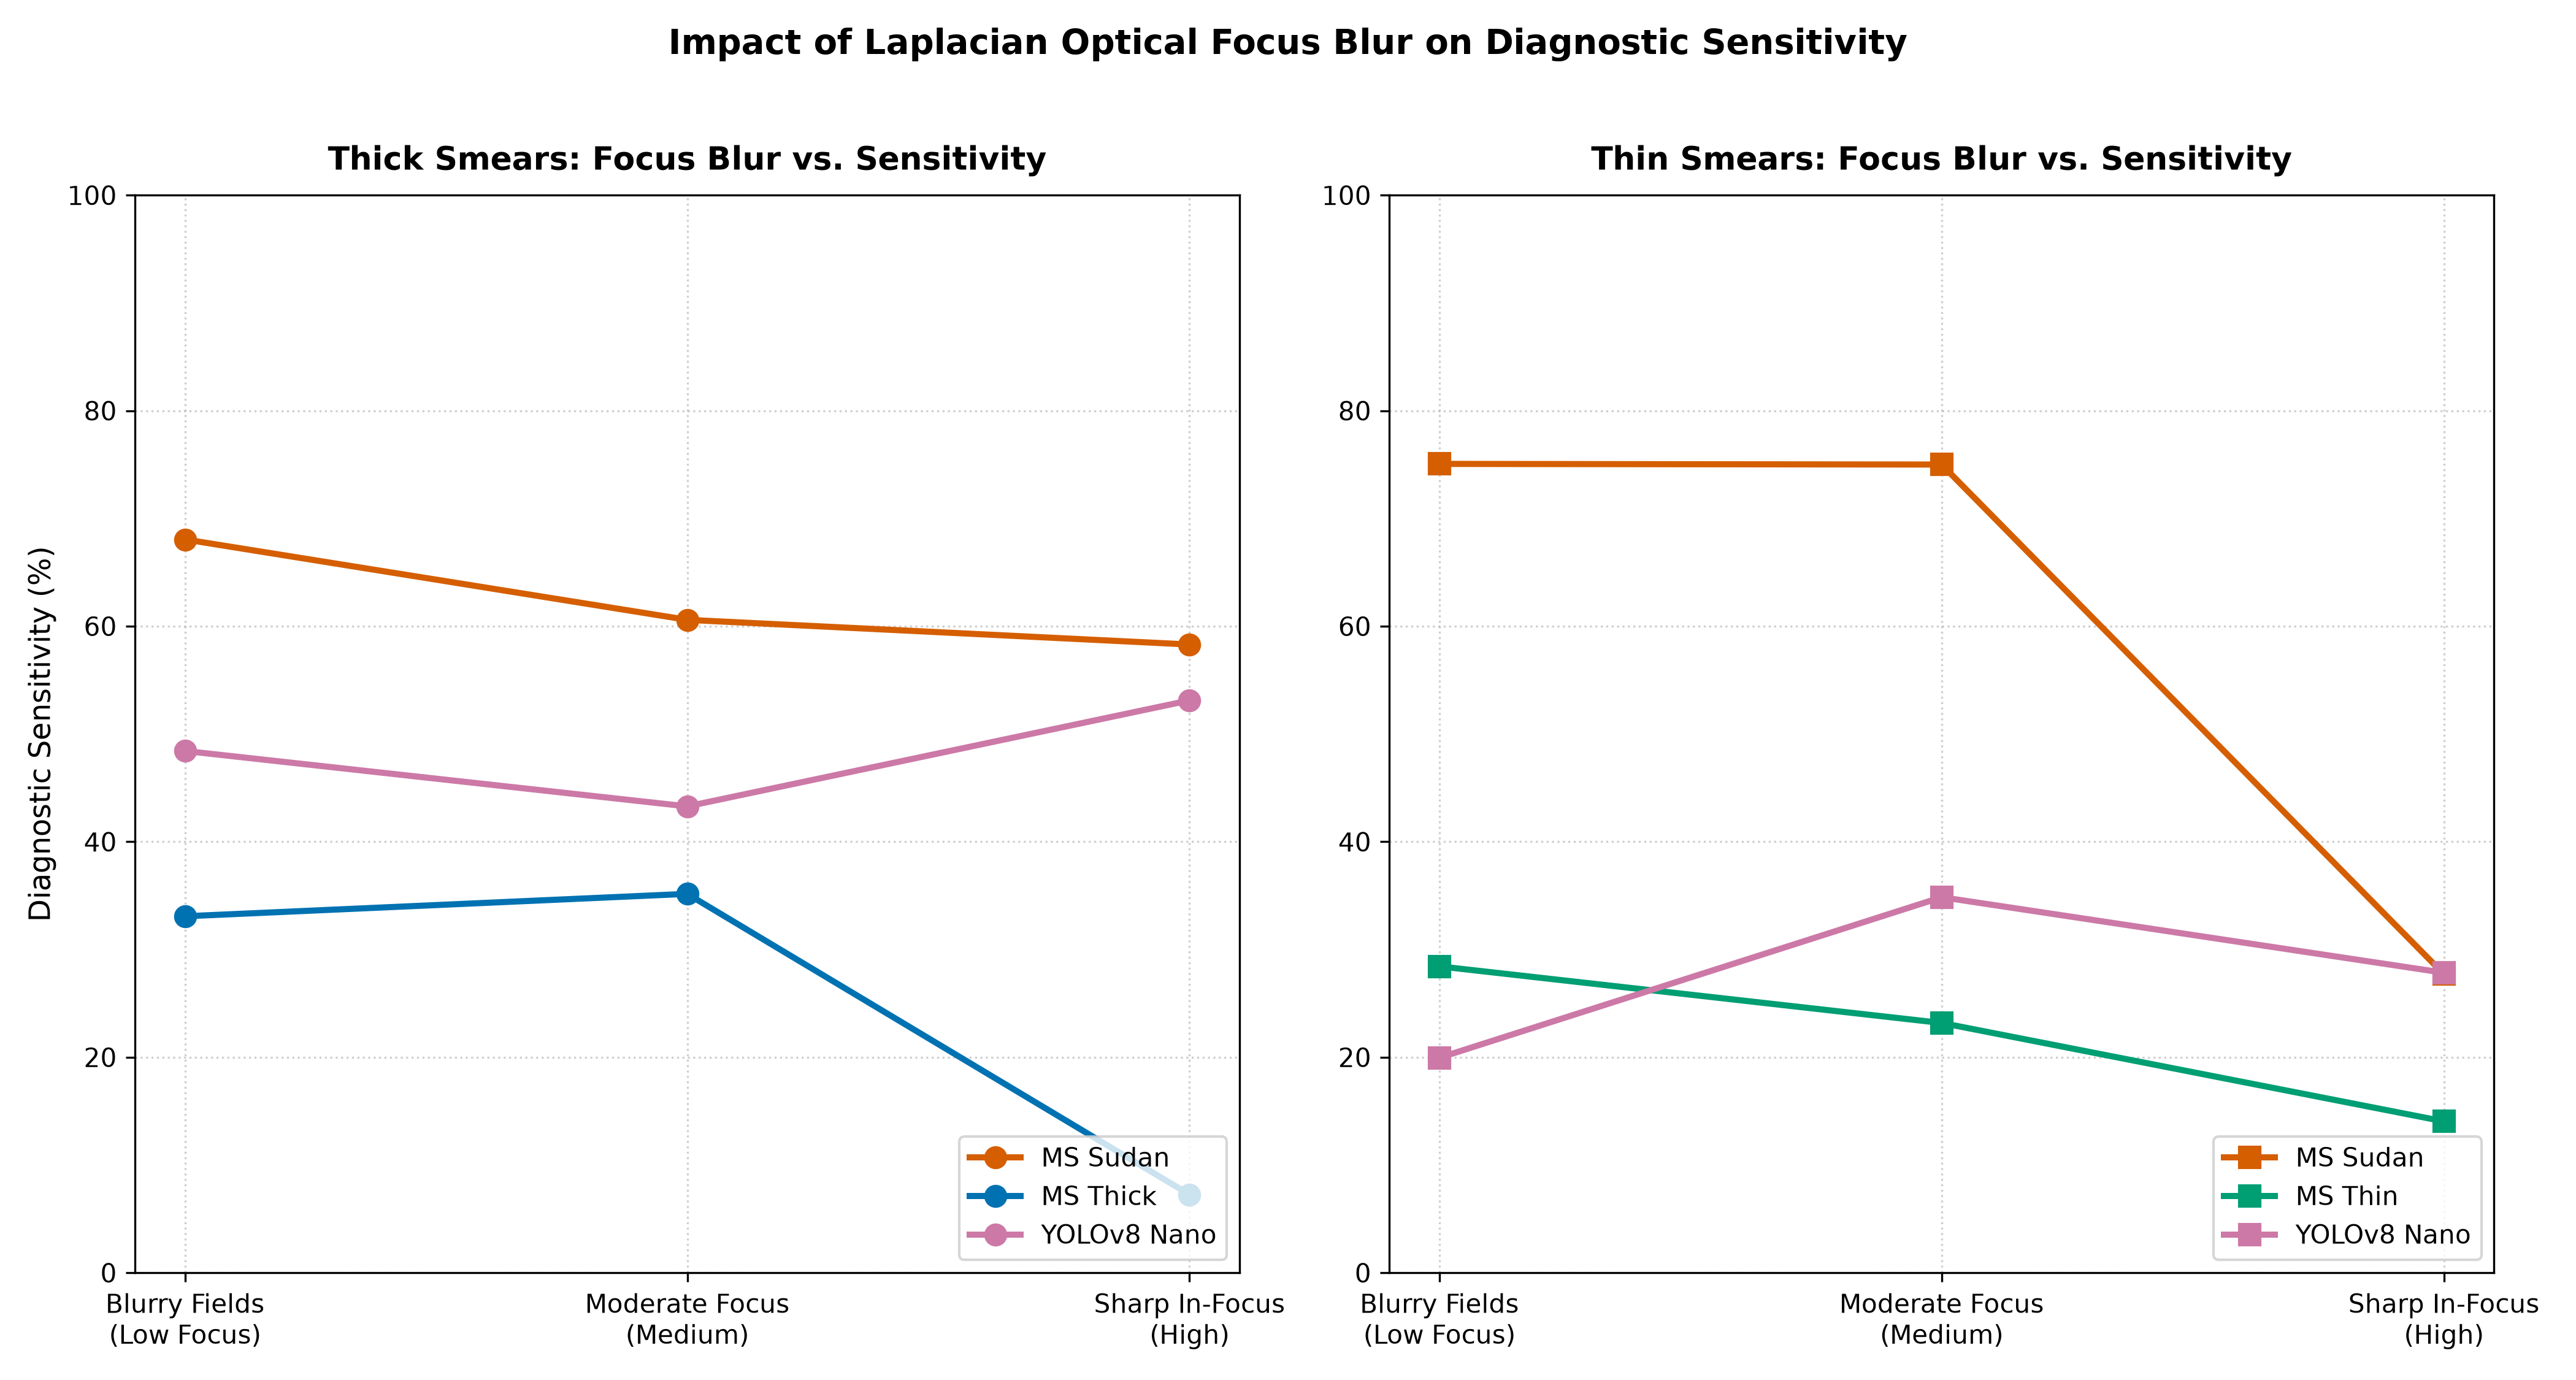
\includegraphics[width=0.95\linewidth]{figures/fig3_optical_quality_curves.png}
\caption{Impact of optical focus blur on diagnostic sensitivity. Severe defocus blur impairs visual feature resolution, with sensitivity degrading by up to 23.8\% in thin smear monolayers, demonstrating the critical necessity of an automated pre-inference focus gate.}
\label{fig:optical_quality_curves}
\end{figure}

\subsection{Regional Fine-Tuning: Bridging the Generalization Gap (RQ5)}
To evaluate RQ5 and determine whether domain-specific regional adaptation overcomes zero-shot degradation, models undergo fine-tuning using the stratified 70/15/15 multi-center split. Table~\ref{tab:finetuning} benchmarks zero-shot baselines against regionally adapted checkpoints.

\begin{table}[htbp]
\centering
\small
\caption{Comparative Diagnostic Performance: Zero-Shot vs. Regionally Fine-Tuned Models across West African Smears (RQ5).}
\label{tab:finetuning}
\resizebox{\linewidth}{!}{%
\begin{tabular}{lcccccc}
\toprule
\textbf{Architecture \& Modality} & \multicolumn{2}{c}{\textbf{Sensitivity (\%)}} & \multicolumn{2}{c}{\textbf{Specificity (\%)}} & \bm{$\Delta F_1$} & \textbf{WHO Level-1} \\
\cmidrule(lr){2-3} \cmidrule(lr){4-5}
 & \textbf{Zero-Shot} & \textbf{Fine-Tuned} & \textbf{Zero-Shot} & \textbf{Fine-Tuned} & & \textbf{Status} \\
\midrule
\multicolumn{7}{l}{\textit{Thick Smear Evaluation Cohort ($N = 3,902$)}} \\
MalariaScreener\_Sudan & 63.88\% & \textit{[Pending FT]} & 55.69\% & \textit{[Pending FT]} & \textit{[---]} & \textit{[Pending FT]} \\
MalariaScreener\_Thick & 30.29\% & \textit{[Pending FT]} & 83.18\% & \textit{[Pending FT]} & \textit{[---]} & \textit{[Pending FT]} \\
fbononi\_YOLOv8        & 47.13\% & \textit{[Pending FT]} & 96.92\% & \textit{[Pending FT]} & \textit{[---]} & \textit{[Pending FT]} \\
\midrule
\multicolumn{7}{l}{\textit{Thin Smear Evaluation Cohort ($N = 2,555$)}} \\
MalariaScreener\_Sudan & 53.64\% & \textit{[Pending FT]} & 43.74\% & \textit{[Pending FT]} & \textit{[---]} & \textit{[Pending FT]} \\
MalariaScreener\_Thin  & 20.27\% & \textit{[Pending FT]} & 57.96\% & \textit{[Pending FT]} & \textit{[---]} & \textit{[Pending FT]} \\
fbononi\_YOLOv8        & 28.23\% & \textit{[Pending FT]} & 68.89\% & \textit{[Pending FT]} & \textit{[---]} & \textit{[Pending FT]} \\
\bottomrule
\end{tabular}%
}
\end{table}

% ── SECTION 4: DISCUSSION ───────────────────────────────────
\section{Discussion}
\label{sec:discussion}

\userinput{Explain in your own words what the numbers in Tables 1--5 mean clinically and technically. Below are the 5 guided discussion tracks for your input:}

\subsection{Deconstructing the African Regional Advantage (RQ1)}
\userinput{Why does the Sudan-trained model achieve superior sensitivity compared to the Asian models on West African smears? What differences in staining, Giemsa intensity, or slide preparation explain this?}

\subsection{The Modality Transfer Cliff: Why YOLOv8 Collapses on Thin Smears (RQ2)}
\userinput{Explain why YOLOv8 dropped significantly on thin smears while MobileNetV2 remained stable. How do intact red blood cell rings confuse the object detector's bounding box proposals?}

\subsection{Geographic \& Hardware Variance Across Accra, Osun, and Kano (RQ3)}
\userinput{What differences did you observe between the three hospital datasets? How did camera phone optics or regional infection types (e.g. rouleaux in Kano) affect model predictions?}

\subsection{Mandating Pre-Inference Hardware Quality Gates (RQ4)}
\userinput{Why can't health centers deploy these models without automated blur pre-filters? What happens when a doctor trusts a model running on an out-of-focus slide?}

\subsection{Efficacy of Regional Fine-Tuning vs. Zero-Shot Transfer (RQ5)}
\userinput{Discuss how regional fine-tuning shifts the clinical utility frontier (RQ5). Does local calibration justify the data collection and computational costs for resource-limited labs?}

\subsection{Study Limitations}
\userinput{What are the practical limitations of our study? (e.g., lack of PCR ground truth confirmation, reliance on optical microscopy labels, specific smartphone camera models).}

% ── SECTION 5: CONCLUSION ───────────────────────────────────
\section{Conclusion \& Policy Recommendations}
\label{sec:conclusion}
\userinput{What are your final recommendations for the Ministry of Health, Ghana FDA, and clinicians adopting automated malaria AI in Africa?}

\section*{Data \& Code Availability}
The complete WAM-Bench evaluation pipeline, model wrappers, optical quality manifests, and reproducibility scripts are publicly available at: \url{https://github.com/wilfredasumboya/Malaria-Models-Evaluations}.

\bibliographystyle{plainnat}
\bibliography{references}

\end{document}
